\subsection{OpenMP benchmark}\label{subsec:openmp}

This subsection reports the parallel scaling analysis performed with OpenMP directives-based paradigm. These benchmarks have been done on a \emph{dual Intel(R) Xeon(R) CPU X5650} exacores workstation for a total of 12 physical cores, coupled with 24GB of RAM. In order to perform an accurate analysis 4 different codes have considered:

\begin{itemize}
  \item FOODIE-aware codes:
    \begin{itemize}
      \item serial code;
      \item OpenMP-enabled code;
      \end{itemize}
  \item procedural codes without using FOODIE library:
    \begin{itemize}
      \item serial code;
      \item OpenMP-enabled code;
      \end{itemize}
  \end{itemize}

These codes (see appendix \ref{sec:euler-1D-OpenMP-API} for the implementation details) have been compiled by means of the GNU gfortran compiler v5.2.0 with \emph{-O2 -fopenmp} compilation flags.

The Euler conservation laws are integrated for 10 time steps by means of the TVD RK(5,4) solver: the measured CPU time used for computing the scaling efficiencies is the average of the 10 integrations, thus representing the mean CPU time for computing one time step integration.

\begin{figure}[!ht]
  \centering
  \begin{subfigure}[b]{0.85\textwidth}
    \centering
    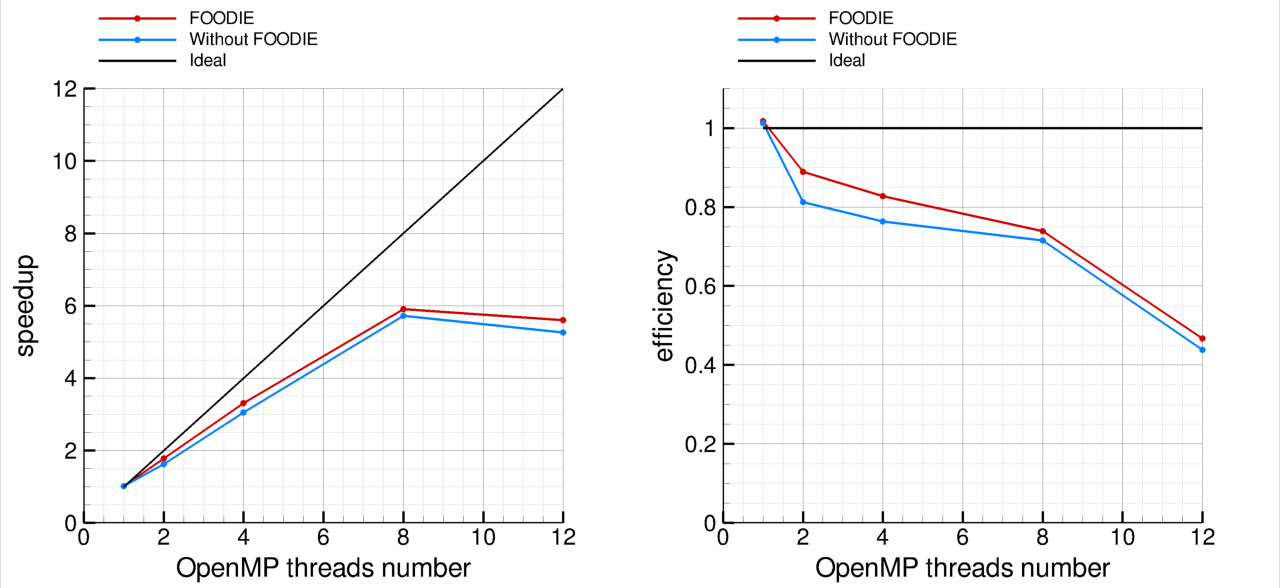
\includegraphics[width=1.00\textwidth]{openmp_benchmark/euler-1D-openmp/strong-scaling-comparison.png}
    \caption{Strong scaling, number of cells 100000}\label{fig:strong-scaling-openmp}
  \end{subfigure}\\
  \begin{subfigure}[b]{0.85\textwidth}
    \centering
    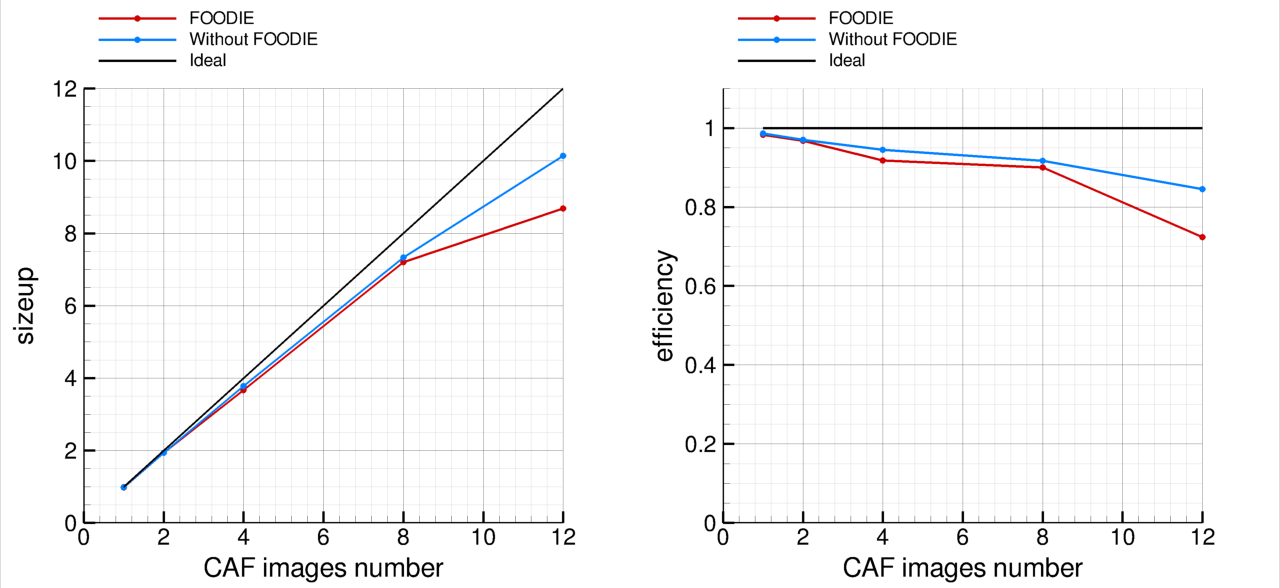
\includegraphics[width=1.00\textwidth]{openmp_benchmark/euler-1D-openmp/weak-scaling-comparison.png}
    \caption{Weak scaling, minimum number of cells 10000}\label{fig:weak-scaling-openmp}
  \end{subfigure}\\
  \caption{Scaling efficiency with OpenMP programming model}\label{fig:scaling-openmp}
\end{figure}

For the strong scaling, the benchmark has been conducted with 100000 finite volumes. Figure \ref{fig:strong-scaling-openmp} summarizes the strong scaling analysis: it shows that FOODIE-based code scales similarly to the baseline code without FOODIE.

For the weak scaling the minimum size is 10000 finite volumes and the size is scaled linearly with the OpenMP threads, thus $N_{12} = 120000$ cells. Figure \ref{fig:weak-scaling-openmp} summarizes the weak scaling analysis and it essentially confirms that FOODIE-based code scales similarly to the baseline code without FOODIE.

Both strong and weak scaling analysis point out that for the computing architecture considered the parallel scaling is reasonable up to 8 cores: using 12 cores the measured efficiencies become unsatisfactory, reducing below the 50\%.

To complete the comparison, the absolute CPU-time consumed by the two families of codes (with and without FOODIE) must be considered. Table \ref{tab:openmp-results} summarizes the benchmarks results. As shown, procedural and FOODIE-aware codes consume a very similar CPU-time for both the strong and the weak benchmarks. The same results are shown in figure \ref{fig:cpu-time-openmp}. These results prove that the abstraction of FOODIE environment does not degrade the computational efficiency.

\begin{table}[!ht]
  \centering
  \caption{OpenMP benchmarks results\label{tab:openmp-results}}
  \begin{subtable}[b]{0.80\textwidth}
    \centering
    \caption{Strong benchmarks, number of cells 100000\label{tab:openmp-results-strong}}
    \resizebox{1.00\textwidth}{!}{%
    \begin{tabular}{ccccc}
      {\sc Number of OpenMP threads} & \multicolumn{4}{c}{\sc CPU time for 1 time step integration}              \\
      \hline
                                     & FOODIE serial & FOODIE parallel & procedural serial & procedural parallel \\
      \cmidrule{2-5}
      1                              & 1.2941        & 1.2942          & 1.2820            & 1.2769              \\
      2                              & /             & 0.7472          & /                 & 0.7784              \\
      4                              & /             & 0.3988          & /                 & 0.4218              \\
      8                              & /             & 0.2185          & /                 & 0.2559              \\
      12                             & /             & 0.2352          & /                 & 0.2272              \\
      \hline
    \end{tabular}}
  \end{subtable}\\
  \begin{subtable}[b]{0.80\textwidth}
    \centering
    \caption{Weak benchmarks, minimum number of cells 10000\label{tab:openmp-results-weak}}
    \resizebox{1.00\textwidth}{!}{%
    \begin{tabular}{cccccc}
      {\sc Number of OpenMP threads} & {\sc Number of Cells} & \multicolumn{4}{c}{\sc CPU time for 1 time step integration} \\
      \hline
                                     &                       & FOODIE serial & FOODIE parallel & procedural serial & procedural parallel \\
      \cmidrule{3-6}
      1                              & 10000                 & 0.1496        & 0.1419          & 1.2820            & 1.2769              \\
      2                              & 20000                 & /             & 0.1643          & /                 & 0.7784              \\
      4                              & 40000                 & /             & 0.1671          & /                 & 0.4218              \\
      8                              & 80000                 & /             & 0.1752          & /                 & 0.2559              \\
      12                             & 120000                & /             & 0.2883          & /                 & 0.2272              \\
      \hline
    \end{tabular}}
  \end{subtable}
\end{table}

\begin{figure}[!ht]
  \centering
  \begin{subfigure}[b]{0.45\textwidth}
    \centering
    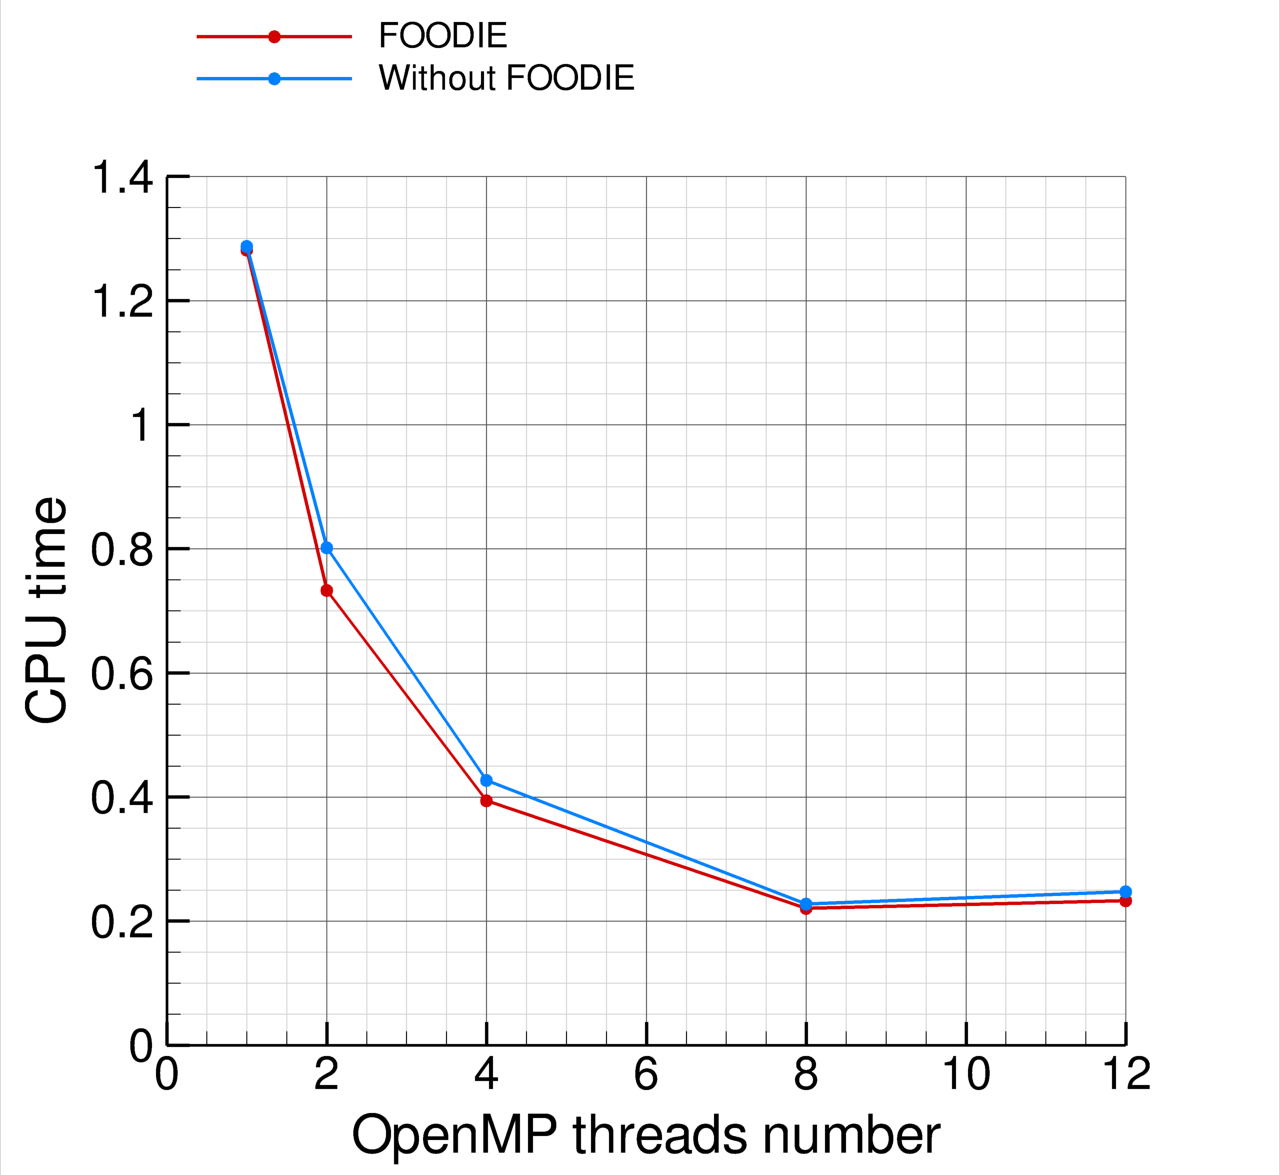
\includegraphics[width=1.00\textwidth]{openmp_benchmark/euler-1D-openmp/strong-cpu-time-comparison.png}
    \caption{Strong benchmark, number of cells 100000}\label{fig:strong-cpu-time-openmp}
  \end{subfigure}\quad%
  \begin{subfigure}[b]{0.45\textwidth}
    \centering
    \includegraphics[width=1.00\textwidth]{openmp_benchmark/euler-1D-openmp/weak-cpu-time-comparison.png}
    \caption{Weak benchmark, minimum number of cells 10000}\label{fig:weak-cpu-time-openmp}
  \end{subfigure}\\
  \caption{CPU time consumed with OpenMP programming model}\label{fig:cpu-time-openmp}
\end{figure}

